% vim: set tw=78 sts=2 sw=2 ts=8 aw et ai:

In order to explain the algorithms used for determining historical relevance, let's first analyze a typical time series, using as example a word that carries a heavy influence on history: war.

\begin{figure*}[ht]
\centering
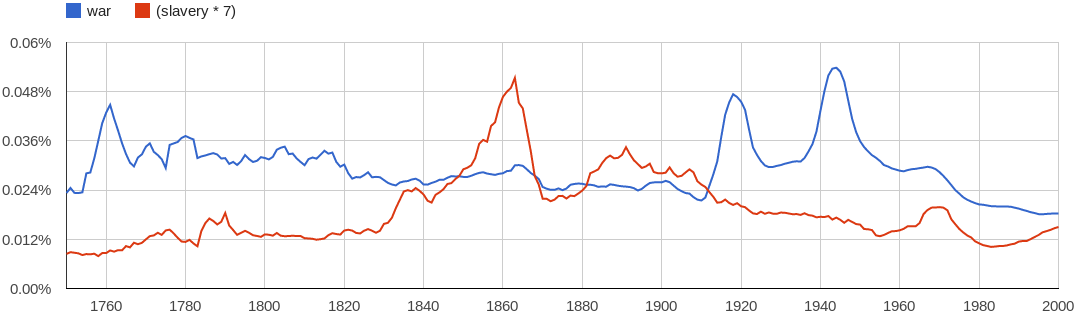
\includegraphics[max size={0.7 \textwidth}{0.7 \textheight}]{war-series}
\caption{Ngram time series for war}
\label{fig:war-series}
\end{figure*}

Taking a look at Figure~\ref{fig:war-series}, the first feature of the plot that can be noticed is the presence of several well-defined peaks. They can be immediately connected with historic events: the first peak, between $1755$ and $1765$, corresponds to the Seven Years' War; the second one, between $1910$ and $1926$, is clearly caused by World War I; the third one, between $1936$ and $1953$, is determined by World War II.

However, a closer inspection reveals the presence of further peak-like shapes, some of which can be identified with major wars in history. Between $1775$ and $1783$ took place the American Revolutionary War. Between $1860$ and $1871$ one can note another peak most probably corresponding to the American Civil War. More recently, between $1961$ and $1978$, there is a shape vaguely resembling a peak most likely generated by the Vietnam War. One must note that the shape of a singular plot can only reveal so much information, but by determining historical relevance for different n-grams and correlating the results, one can viably get a picture of a historic event.

\begin{figure*}[ht]
\centering
\includegraphics[max size={0.7 \textwidth}{0.7 \textheight}]{comparative-series}
\caption{Ngram time series for atomic, trench and slavery}
\label{fig:comparative-series}
\end{figure*}

As a prime example of the above idea, Figure~\ref{fig:comparative-series} presents a comparative analysis of the following 3 n-grams: atomic, trench and slavery. Firstly, slavery has a very sharp triangular peak between $1842$ and $1871$, which includes the American Civil War, known for the fact it had slavery as a core issue. Secondly, trench has a significant peak between $1911$ and $1925$, corresponding to World War I, known for the heavy use of trench warfare. Lastly, atomic also has a wide peak between $1939$ and $1972$, motivated by the development of the atomic bomb, its use in World War II and its potential use in the Cold War.

For this analysis to be tractable on the large amounts of data available in the corpus, one must come up with an algorithm for peak detection. Depending on the complexity of the algorithm, a subset of the corpus may have to be left out from processing. Intuitively, one should leave out the least frequent n-grams, the heuristic being that very rare words are pretty unlikely to be connected with a major historic event, thus not affecting the quality of the results. A further requirement for the algorithm is the capability of meaningfully characterizing a peak. Thus, it also needs to quantitatively measure the historical relevance of that peak. For example, the three large peaks of the n-gram war should be assigned a high historical relevance. Furthermore, the value of the historical relevance needs not be constant over the entire peak. Instead, advanced schemes can use a variable historical relevance, perhaps assigning more to the center of the peak and less to the outskirts of the peak.

\subsubsection{Double Change Peak Detection}

Arguably the simplest way of detecting peaks is by making use of the fact that peaks usually consist of a period of abrupt increase, followed by another period of abrupt decrease. A computationally inexpensive method for doing this is detecting periods of time marked by a double change of the time series in the same direction, either increasing or decreasing.

Formally, we say that a time series $\left\{ s_{i, t} \right\}$ suffers a double increase or decrease if it increases or decrease twice consecutively. Furthermore, the magnitude of that increase (Equation~\ref{eq:double-increase}) or decrease (Equation~\ref{eq:double-decrease}) at time $t$ is defined as the maximum $x \in \left[ 0, 1 \right]$ that satisfies one of the following equations:

\begin{align}
\label{eq:double-increase}
s_{i, t} > \left( 1 + x \right) s_{i, t - 1}, \, s_{i, t + 1} > \left( 1 + x \right) s_{i, t}
\\
\label{eq:double-decrease}
s_{i, t} < \left( 1 - x \right) s_{i, t - 1}, \, s_{i, t + 1} < \left( 1 - x \right) s_{i, t}
\end{align}

One problem that may appear with these definitions is that, for example, during the ascent part of the peak, at often times the increase rate will randomly dip below a certain threshold, causing the algorithm to miss valuable information. To this end, the magnitude of a single increase (Equation~\ref{eq:single-increase}) or of a single decrease (Equation~\ref{eq:single-decrease}) at time $t$ is defined as the maximum $x \in \left[ 0, 1 \right]$ that satisfies one of:

\begin{align}
\label{eq:single-increase}
s_{i, t} &> \left( 1 + 2x \right) s_{i, t - 1}
\\
\label{eq:single-decrease}
s_{i, t} &< \left( 1 - 2x \right) s_{i, t - 1}
\end{align}

The latter two notions use a factor of $2x$ in the formulas, the reasoning being that although we don't want to miss any potential peaks, single changes in the time series can sometimes not be part of a peak and therefore it should be harder for them to achieve a certain magnitude.

The magnitude $m_{i, t}$ of the change around a point $t$ in a time series $\left\{ s_{i, t} \right\}$ is defined as the maximum between the magnitude of the double change and the magnitude of the single change at that point. The historical relevance is proportional to the magnitude $m_{i, t}$, with an artificial cap imposed to avoid overemphasizing new words that grow explosively:

\begin{align}
\label{eq:double-change-relevance}
r_{i, t} &= \min \left( \left\lfloor 10 m_{i, t} \right\rfloor, 9 \right).
\end{align}

\subsubsection{Linear Model Peak Detection}

Drawing on the previous idea of periods of abrupt increase and decrease, one can also use a linear model for approximating portions of the time series. The core of this approach is to fit lines to the graph of the time series using linear regression, by considering larger and larger intervals until the error rises above a given threshold. Of course, the series must initially be normalized by using the standard score.

\begin{algorithm}

\begin{algorithmic}[1]
\For { $i \in 1 \to \left| \textrm{Words} \right|$ }
    \State $u \gets 1500$
    \For { $t \in 1501 \to 2008$ }
        \State $a, b, err \gets \textrm{lm} \left( \left\{ s_{i, k} \right\}_{k = u}^t \right)$
        \If { $\log(err) >= -5$ }
            \State $m_i \left( \left[ u, t \right] \right) \gets 2 \cdot \left( 3 + \log \left| a \right| \right)$
            \State $u \gets t$
        \EndIf
    \EndFor
\EndFor
\end{algorithmic}

\caption{Linear Model Peak Detection Algorithm}
\label{alg:linear-model}

\end{algorithm}

As can be noticed in Algorithm~\ref{alg:linear-model}, upon finding a maximal interval fitted by a line within a small error, the magnitude of the change on that interval is defined as a linear function of the logarithm of the slope. This choice is motivated by the wide range of values that the slope can take, forming a sort of heavy-tailed distribution. The historical relevance for $w_i$ is then simply computed as follows: $r_{i, t} = \max \left( \left\lfloor m_{i, t} \right\rfloor, 0 \right)$.

\subsubsection{Gaussian Model Peak Detection}

Another completely different idea for peak detection is to notice that peaks are usually shaped like a Gaussian distribution. Let us consider a time interval $\left[ l, r \right] \subseteq \left[ 1500, 2008 \right]$ and the time series for some word $w_i$ on that interval, $\left\{ s_{i, t} \right\}_{t=l}^{r}$. Initially, one must normalize the series to get a probability distribution:

\begin{align}
\label{eq:gaussian-normalization}
g_{i, t} &= \frac{s_{i, t} - \min_{p \in \overline{l, r}} s_{i, p}}{\sum_{q = l}^{r} \left( s_{i, q} - \min_{p \in \overline{l, r}} s_{i, p} \right)}.
\end{align}

This is approximated by a normal distribution $N \left( \mu, \sigma \right)$ with the following parameters:

\begin{align}
\label{eq:mu-gaussian-model}
\mu &= \sum_{t=l}^{r} g_{i, t} t, \\
\label{eq:sigma-gaussian-model}
\sigma^2 &= \sum_{t=l}^{r} g_{i, t} \left( t - \mu \right)^2.
\end{align}

The similarity between $g_{i, t}$ and $N \left( \mu, \sigma \right)$ is computed using the earth mover's distance introduced in \newcite{rubner98metric}. Although the former probability distribution is discrete, while the latter is continuous, we shall nonetheless assume that the latter is also discrete by considering only its values in the points $t \in \overline{l, r}$. As we find ourselves in the one-dimensional case, the problem can be solved using a greedy algorithm that runs in linear time. When modeling peaks with Gaussian distributions, we unfortunately have to consider all possible intervals $\left[ l, r \right] \subseteq \left[ 1500, 2008 \right]$, which leads to cubic complexity in the number of years analyzed. This can be improved by using a heuristic to decide if a probability distribution even remotely looks like a Gaussian bell. One such possible measure is kurtosis, which is defined in terms of the fourth moment about the mean $\mu_4$:

\begin{align}
\label{eq:kurtosis}
\gamma_2 &= \frac{\mu_4}{\sigma^4} - 3.
\end{align}

As evidenced in \newcite{balanda88kurtosis}, in the case of symmetric distributions, kurtosis can be viewed as an approximate measure of peakedness, with the normal distribution having a kurtosis of $0$, so one can impose a tight limit on this value, such as $0.05$. Fortunately, kurtosis can be computed in constant time for any interval, using trivial preprocessing of partial sums.

After that, from the remaining intervals we select the ones that have an earth mover's distance to their corresponding Gaussian distributions lower than $0.3$. A potential problem that can appear is that the intervals may intersect. This can be avoided by first sorting the intervals in increasing order of the earth mover's distance and then processing them one by one. Intervals that intersect previously processed ones are simply ignored, which both ensures that the intervals are disjoint and that only the highest quality peaks are chosen.

Now we compute the magnitude of the change corresponding to an interval $\left[ l, r \right]$ as the percentage with which the Gaussian peak increases from its smallest value to its largest value. The minimum value is computed as a statistic from the original series, while the largest value is derived from the largest value of the Gaussian distribution:

\begin{align}
\label{eq:gaussian-magnitude}
m_i \left( l, r \right) &= \frac{N \left( \mu, \sigma \right) \left( \mu \right) \cdot \sum_{q} \left( s_{i, q} - \min_{p} s_{i, p} \right)}{\min_{p} s_{i, p}}.
\end{align}

One way to define historical relevance in this case is to assign it a constant value on the interval, proportional to the magnitude:

\begin{align}
\label{eq:gaussian-model-constant-relevance}
r_{i, t} &= \left\lfloor 10 \cdot \min \left( m_i \left( l, r \right), 1) \right) \right\rfloor.
\end{align}

An alternative way is to assign variable relevance, such that it also forms a Gaussian bell. The formula, that also includes a widening parameter $w \in \left[ 1, \infty \right)$, is as follows:

\begin{align}
\label{eq:gaussian-model-variable-relevance}
r_{i, t} \left( w \right) &= r_{i, t} \cdot \frac{N \left( \mu, w \sigma \right) \left( t \right)}{N \left( \mu, w \sigma \right) \left( \mu \right)}, \, \forall t \in \left[ l, r \right].
\end{align}

One can note that when $w \to \infty$, Equation~\ref{eq:gaussian-model-variable-relevance} actually converges to Equation~\ref{eq:gaussian-model-constant-relevance}. The idea behind the parameter $w$ is that both extremes are likely to give poor performance: for $w = 1$, too little relevance is assigned to the tails of the distribution, while for $w \to \infty$ too much relevance is assigned to the tails of the distribution. By considering intermediate values one is likely to obtain higher quality results.

\subsubsection{Graphical Analysis}

\begin{figure}[t]
\centering
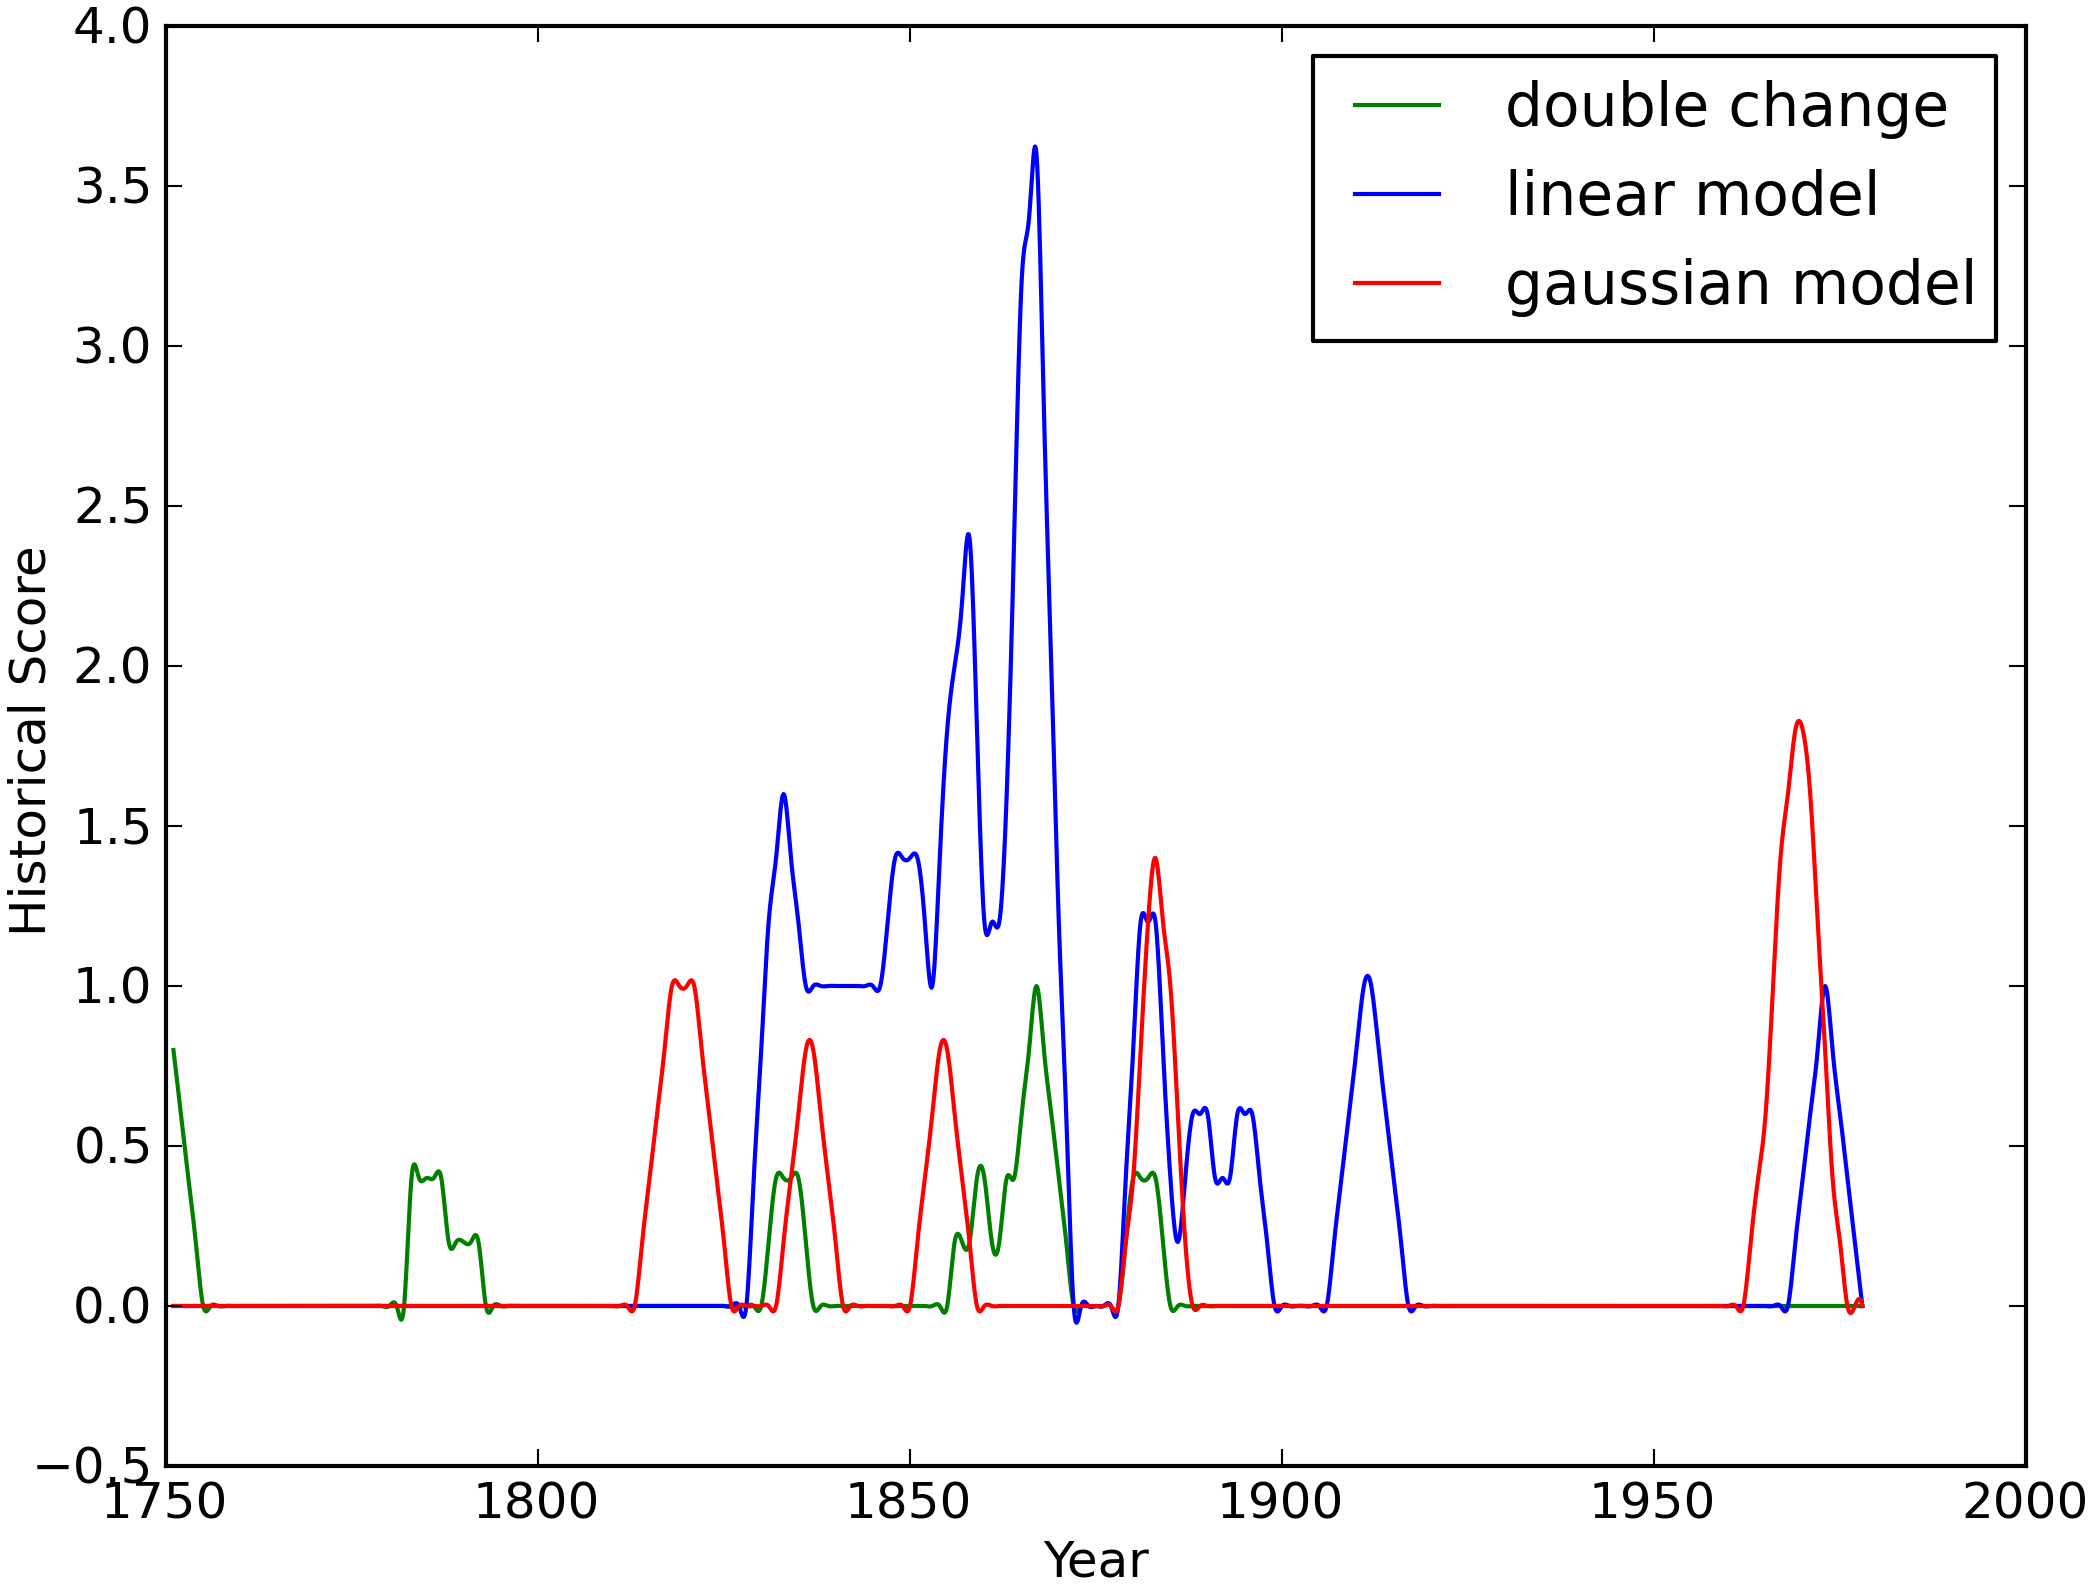
\includegraphics[max size={0.5 \textwidth}{0.5 \textheight}]{slavery-relevance}
\caption{Historical relevance of slavery}
\label{fig:slavery-relevance}
\end{figure}

Of the three algorithms, it cannot be said that one of the them performs the best at detecting and characterizing peaks. However, with the help of an example such as Figure~\ref{fig:slavery-relevance}, one can point the strengths and weaknesses of each of them (for the Gaussian model, the widening parameter used is $w = 2$). As it could be seen in Figure~\ref{fig:comparative-series}, slavery has had two important "historic peaks": the first, between $1842$ and $1871$, includes the American Civil War, while the second, between $1964$ and $1979$, includes the African-American Civil Rights Movement.

The first peak is detected by all three algorithms. The best detection is performed by the linear model, since it can be approximated well by 2 lines. The other algorithms also detect activity in this period, but in 2 distinct intervals. Notably, the second interval detected by the Gaussian model is centered around the American Civil War. The conclusion is that although the linear model is better at detecting triangular peaks, the Gaussian model does a better job at identifying the high point that probably corresponds to a historic event. The double change model is significantly worse than the other two, since it assigns more relevance to the tails of the triangle.

The second peak is detected only by the last two algorithms. Although both reasonably identify the peak, the Gaussian model performs better by considering a slightly larger interval. This is to be expected, as the peak is roughly bell-shaped.

Lastly, the double change model also detects a minor peak centered around $1790$. In that period, the Constitution of the United States was drafted, and one if its highlights was the Three-Fifths Compromise, which stated that for representation purposes, slaves counted as only three-fifths of a person. Thus, although theoretically inferior to the other two algorithms, the double change model has the capability of detecting less important historic events.
